\documentclass{article}
\usepackage[utf8]{inputenc}
\usepackage{graphicx}
\addtolength{\evensidemargin}{-.875in}

\title{122B Spring 2016 \\ Program 2}
\author{Russell Miller and Rylan Schaeffer }
\date{June 2016}

\begin{document}

\maketitle

\section*{Introduction}
Quicksort, Quickselect and Deterministicselect are three algorithms that can be used to select the $k$th smallest element of an unordered list (frequently referred to as an array). We sought to compare their performance relative to list size; to do so, we generated 

\section*{Algorithms and Pseudocode}
\subsection*{Quickselect}
\indent \indent 

\subsection*{Deterministicselect}
\indent \indent 

\subsection*{Quicksort with Select}
\indent \indent Quicksort differ from the two prior algorithms in that it is a sorting algorithm i.e. it rearranges the list in increasing order; to select the $kth$ smallest element, one simply selects the $k$th element from the sorted list.

Quicksort sorts the list using the same principle as Quickselect: an element is selected from the list (called the pivot), and then the list is partitioned into two lists such that all elements in one list are less than the pivot and all elements in the other list are greater than the pivot. But rather than recursing into one of the two new lists as Quickselect does, Quicksort applies the same procedure recursively to both lists. Thus, Quicksort peforms substantially more work than Quickselect.

\section*{Empirical Study}
To investigate the relative performance of Quicksort with Select, Quick Select and Deterministic Select

\section*{Results}
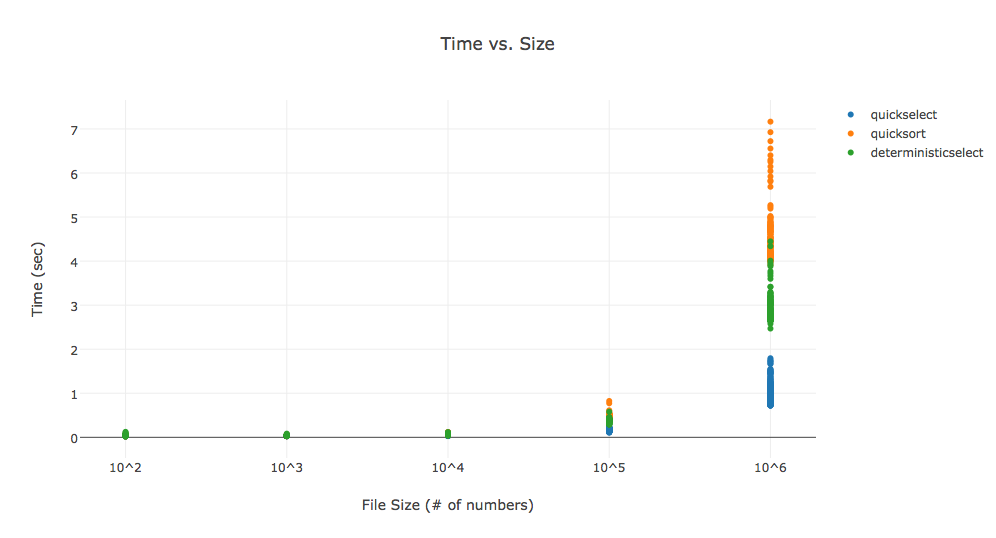
\includegraphics[scale=.4]{results}

\section*{Conclusion}

\section*{Citation}

\end{document}
